%Mars Benchmarks

\subsection{Mars Benchmarks}

The purpose of this benchmark calculation was to demonstrate native FLUKA's ability
to simulate the behavior of the Galactic Cosmic Ray (GCR) on the surface of Mars,
and the fidelity with which we can calculate the dose received at the surface of Mars.
The GCR source code is described in section \ref{SRAGCodes}, and the geometry of
Mars will be described below.

\subsection*{Geometry}
The geometry used in this benchmark calculation consisted of the surface of Mars and
its atmosphere. To generate the geometry of mars, spherical shells were used.
The first sphere modeled the planet and the rest of the spheres modeled the atmospheres.
A region of interest was also defined in the geometry and this was 20 km by 20 km
by 20 km in the x, y and z direction respectively.
The surface of the planet was made of Regolith with composition described in
Appendix \ref{App:A1}.
The atmosphere model consisted of layers of atmosphere with composition described in
Appendix \ref{App:A1} and densities described by the following equation:
\begin{equation}
\label{density}
\rho = \rho_0 *exp(- \frac{z}{H})
\end{equation}
Where $z$ is the height at which we want the density, H is the scale height of the atmosphere,
and $\rho_0 = 2E-5 g/cm^3$.
A script was written in python to write input files that had different number of atmospheric
layers, with its respective average density.

Several models were created and a benchmark calculation was perform in each of them.
This was done with the purpose of understanding if the number of atmosphere layers
significantly changed the dose at the surface of Mars and with what fidelity should the model
be constructed.

A model with 27 and 146 atmospheric layers were first generated and results were compared
(See results below).  Because the results of the benchmark calculation run with the models
described above did not show significant difference, the final model consisted of 20 layers
of atmosphere. This was done as specified by NASA's atmosphere model given in Appendix \ref{App:A1}.

This 20 layer model was presented at the Colorado conference. This model was run a little
different than the previous two models. In this case, the tallies were used were
dose in the first layer and last layers as well as proton, neutron and deuteron fluxes.
This model was also biased by isotope from z = 1 to z = 28 to help sample each isotope better.
The final results of each isotope run was collected together to have one final dose.
This was done with the help of a script created by NASA.

\subsection*{Workflow}
The input file was created in native FLUKA where the source, the geometry specified above,
the number of primaries, the tallies wanted, and any other specification were provided.
The model was then run in a High Throughput Computing system with the aid a CHTC tools work flow.
\subsection*{Results}
Figure \ref{146} shows the dose throughout the atmosphere for 146 layers model                
and figure \ref{27} shows the dose for the 27 layers model.      
\begin{figure}
\centering
\begin{subfigure}[b]{.45\textwidth}
\frame{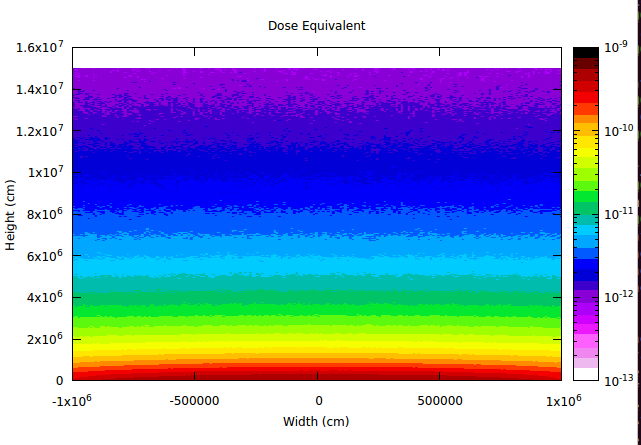
\includegraphics[width=0.85\linewidth,height=5cm]{../figs/dose_95.png}}
\caption{146 layers model}
\label{146}
\end{subfigure}
%
\hspace{0.5cm}
%
\begin{subfigure}[b]{.45\textwidth}
\centering
\frame{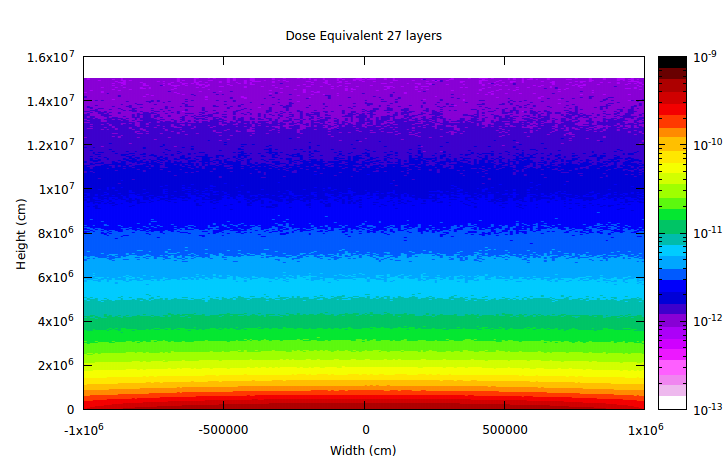
\includegraphics[width=.85\linewidth,height=5cm]{../figs/dose_27.png}}
\caption{27 layers model}
\label{27}
\end{subfigure}
\caption{Dose Deposition}
\end{figure}

\begin{figure}
 \begin{centering}
 \centering
 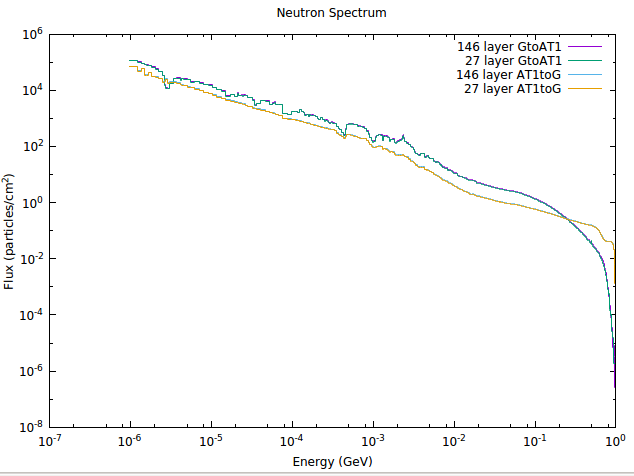
\includegraphics[width=0.4\linewidth,height=5cm]{../figs/neutron.png}
 \caption{Neutron flux for 27 layer and 146 layer model}
 \label{neutron}
 \end{centering}
\end{figure}


The neutron flux was also calculated and compared between the two models.
The differences between them were insignificant. Figure \ref{neutron}
shows the neutron flux from the surface to the first atmosphere and vice-versa.

The results for the 20 layers models was collected for all isotopes and assembled together
by NASA. Some results for individual isotopes will be presented below.
Figure \ref{surface20} shows the flux at the surface of Mars for proton biased source.
\begin{figure}
 \begin{centering}
 \centering
 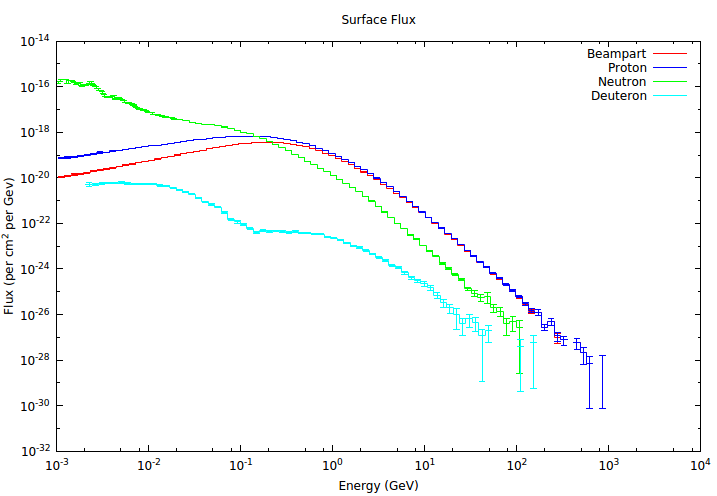
\includegraphics[width=0.4\linewidth,height=5cm]{../figs/surface_z1.png}
 \caption{Flux at the surface of Mars for proton biased source}
 \label{surface20}
 \end{centering}
\end{figure}


